\chapter{Development}

This section describes the chronology of this project's various prototypes. The successes and failures are described, detailing the story of how I arrived at my final product.
% Explain the details of how participants were recruited, how data was collected, recorded, and processed/analyzed, and the timeline over which this process unfolded

\section{First Phase}

The goal of the first prototype was to simply demonstrate how multiple users might interact with a performance using handheld devices. To realize this, I used Wii video game controllers and the Max visual programming software. The final product was a system that allowed seven users to simultaneously manipulate a video loop by performing ``audience-like" motions.


\subsection{Prototyping}

The first step in creating an initial prototype was deciding on the hardware and software that would be used. Wii video game controllers have an abundance of sensors: they contain eleven digital buttons, an infrared sensor, an accelerometer, and a gyroscope (in the newer ``Wii Remote Plus" models), and all of this data can be sent wirelessly to a receiver via Bluetooth technology. In addition to these affordances, due to the console's popularity, the Wii controller is also something that many people are already comfortable moving with -- shaking, waving, swinging. With these considerations, I decided that the Wii controller was a suitable input device for my experiments. Next, I had to find software to process this data. After consulting multiple sources, it became evident that the best way to interface with Wii controllers was to use a combination of two software packages called OSCulator and Max. OSCulator is a program that receives data from devices like MIDI controllers and outputs it using the Open Sound Control (OSC) protocol. Fortunately, it is also preset to communicate with Wii controllers, conveniently displaying live data from each sensor. The OSC data can then be sent to Max, a visual programming environment that is especially useful for handling multimedia. Max is commonly used by musicians and video artists to create highly customized and interactive programs.

My first milestone for this prototype was having a single Wii controller communicate with my computer. Using a program called OSCulator, I was able to read movement and button-push data sent via Bluetooth (see Figure \ref{prototyping1}). From here, the data is sent to a simple Max program (called a ``patcher") that I created. The patcher reads various movement data from the controller and visualizes them as different motions that a typical concertgoer might perform. The motions are: giving a ``thumbs up" or ``thumbs down", swaying arms from side to side, clapping, or doing ``the wave," as shown in Figure \ref{prototyping2}. Visual feedback is provided in the form of illuminated LED objects and moving sliders.

\begin{figure}[t]
	\centering

	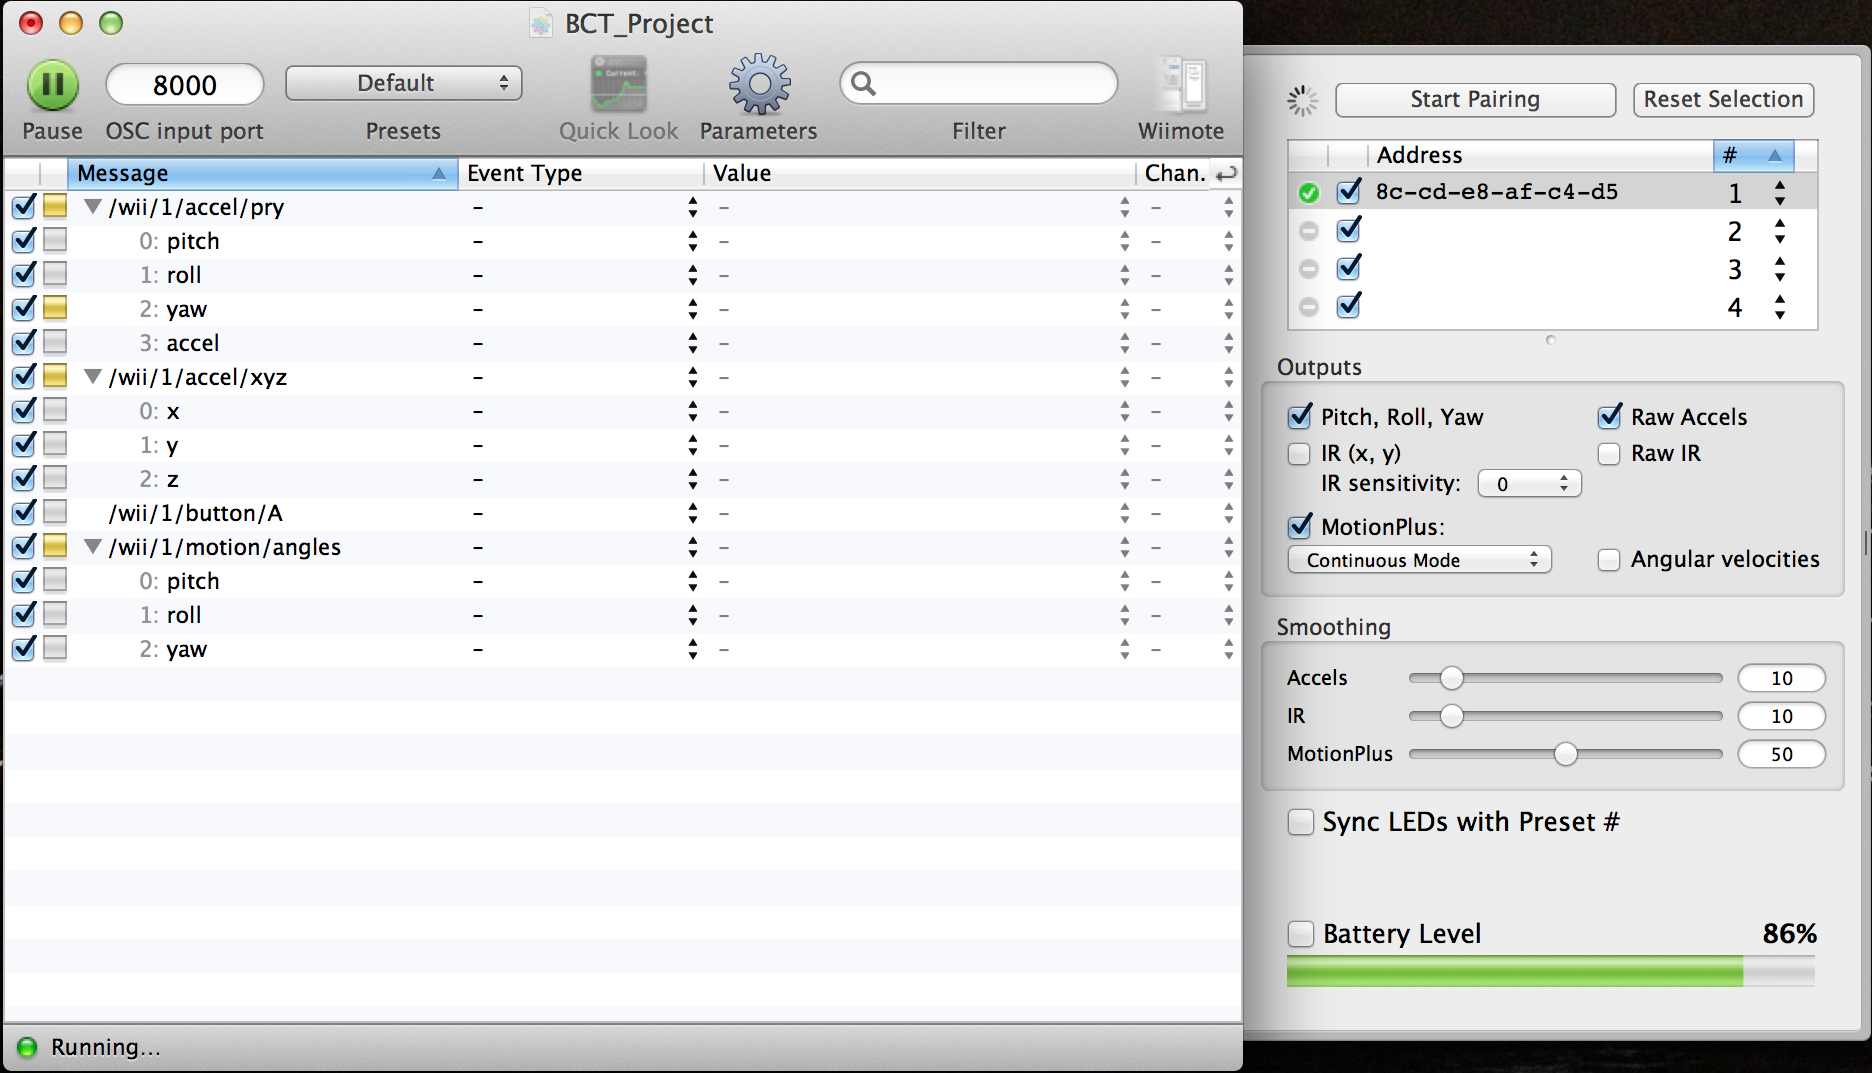
\includegraphics[height=0.3\textwidth]{osculator_1.png}
	\caption{OSCulator software receiving data from one Wii controller}

	\label{prototyping1}
\end{figure}

\begin{figure}[t]
	\centering

	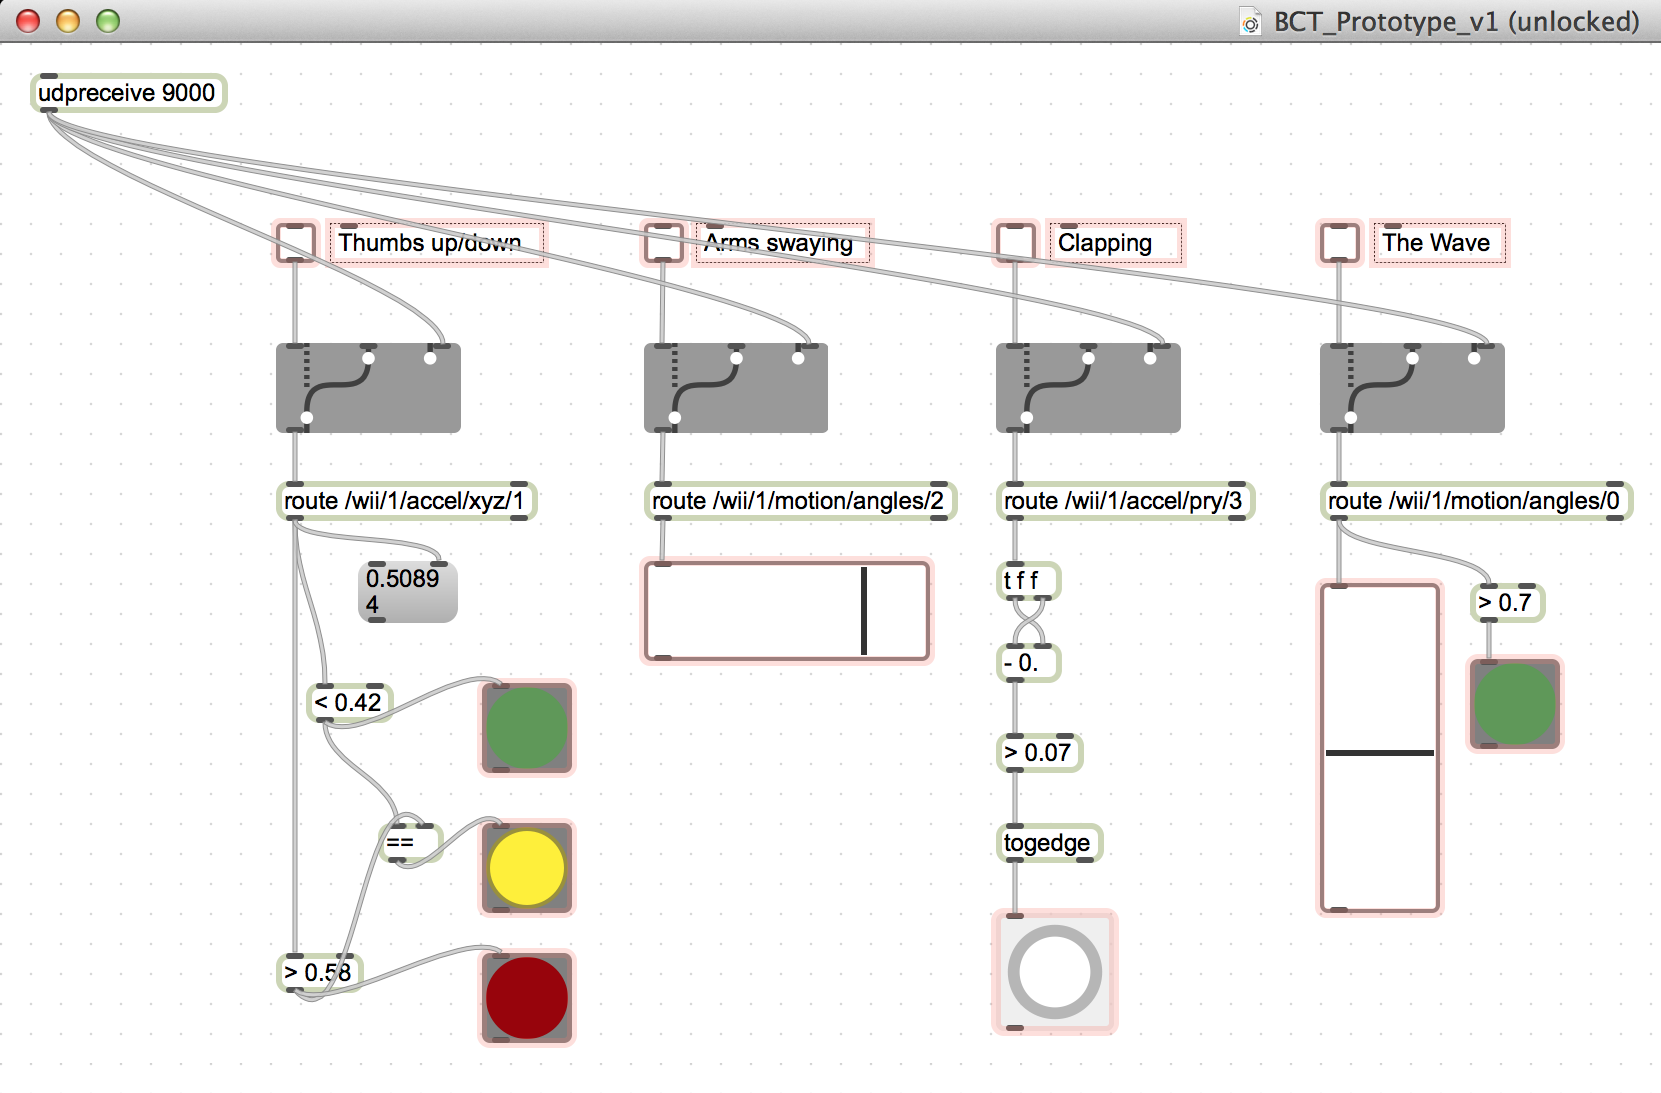
\includegraphics[height=0.3\textwidth]{wiimote_audience.png}
	\caption{First Max patcher}

	\label{prototyping2}
\end{figure}

My second notable achievement was testing the limit of how many Wii controllers would be able to connect to my computer using the current setup. Since my thesis aims to give every member of an audience a new way to communicate, this number would ideally be limitless. The OSCulator software, unfortunately, could only connect to a maximum of seven controllers. However, for the purposes of this prototype, this number is acceptable. To test this, I created a Max patcher to display data from seven Wii controllers. I synced all seven controllers with OSCulator with no issues, and the program worked as expected (see Figure \ref{prototyping3}).

\begin{figure}[t]
	\centering

	\subfloat[Wii controllers]{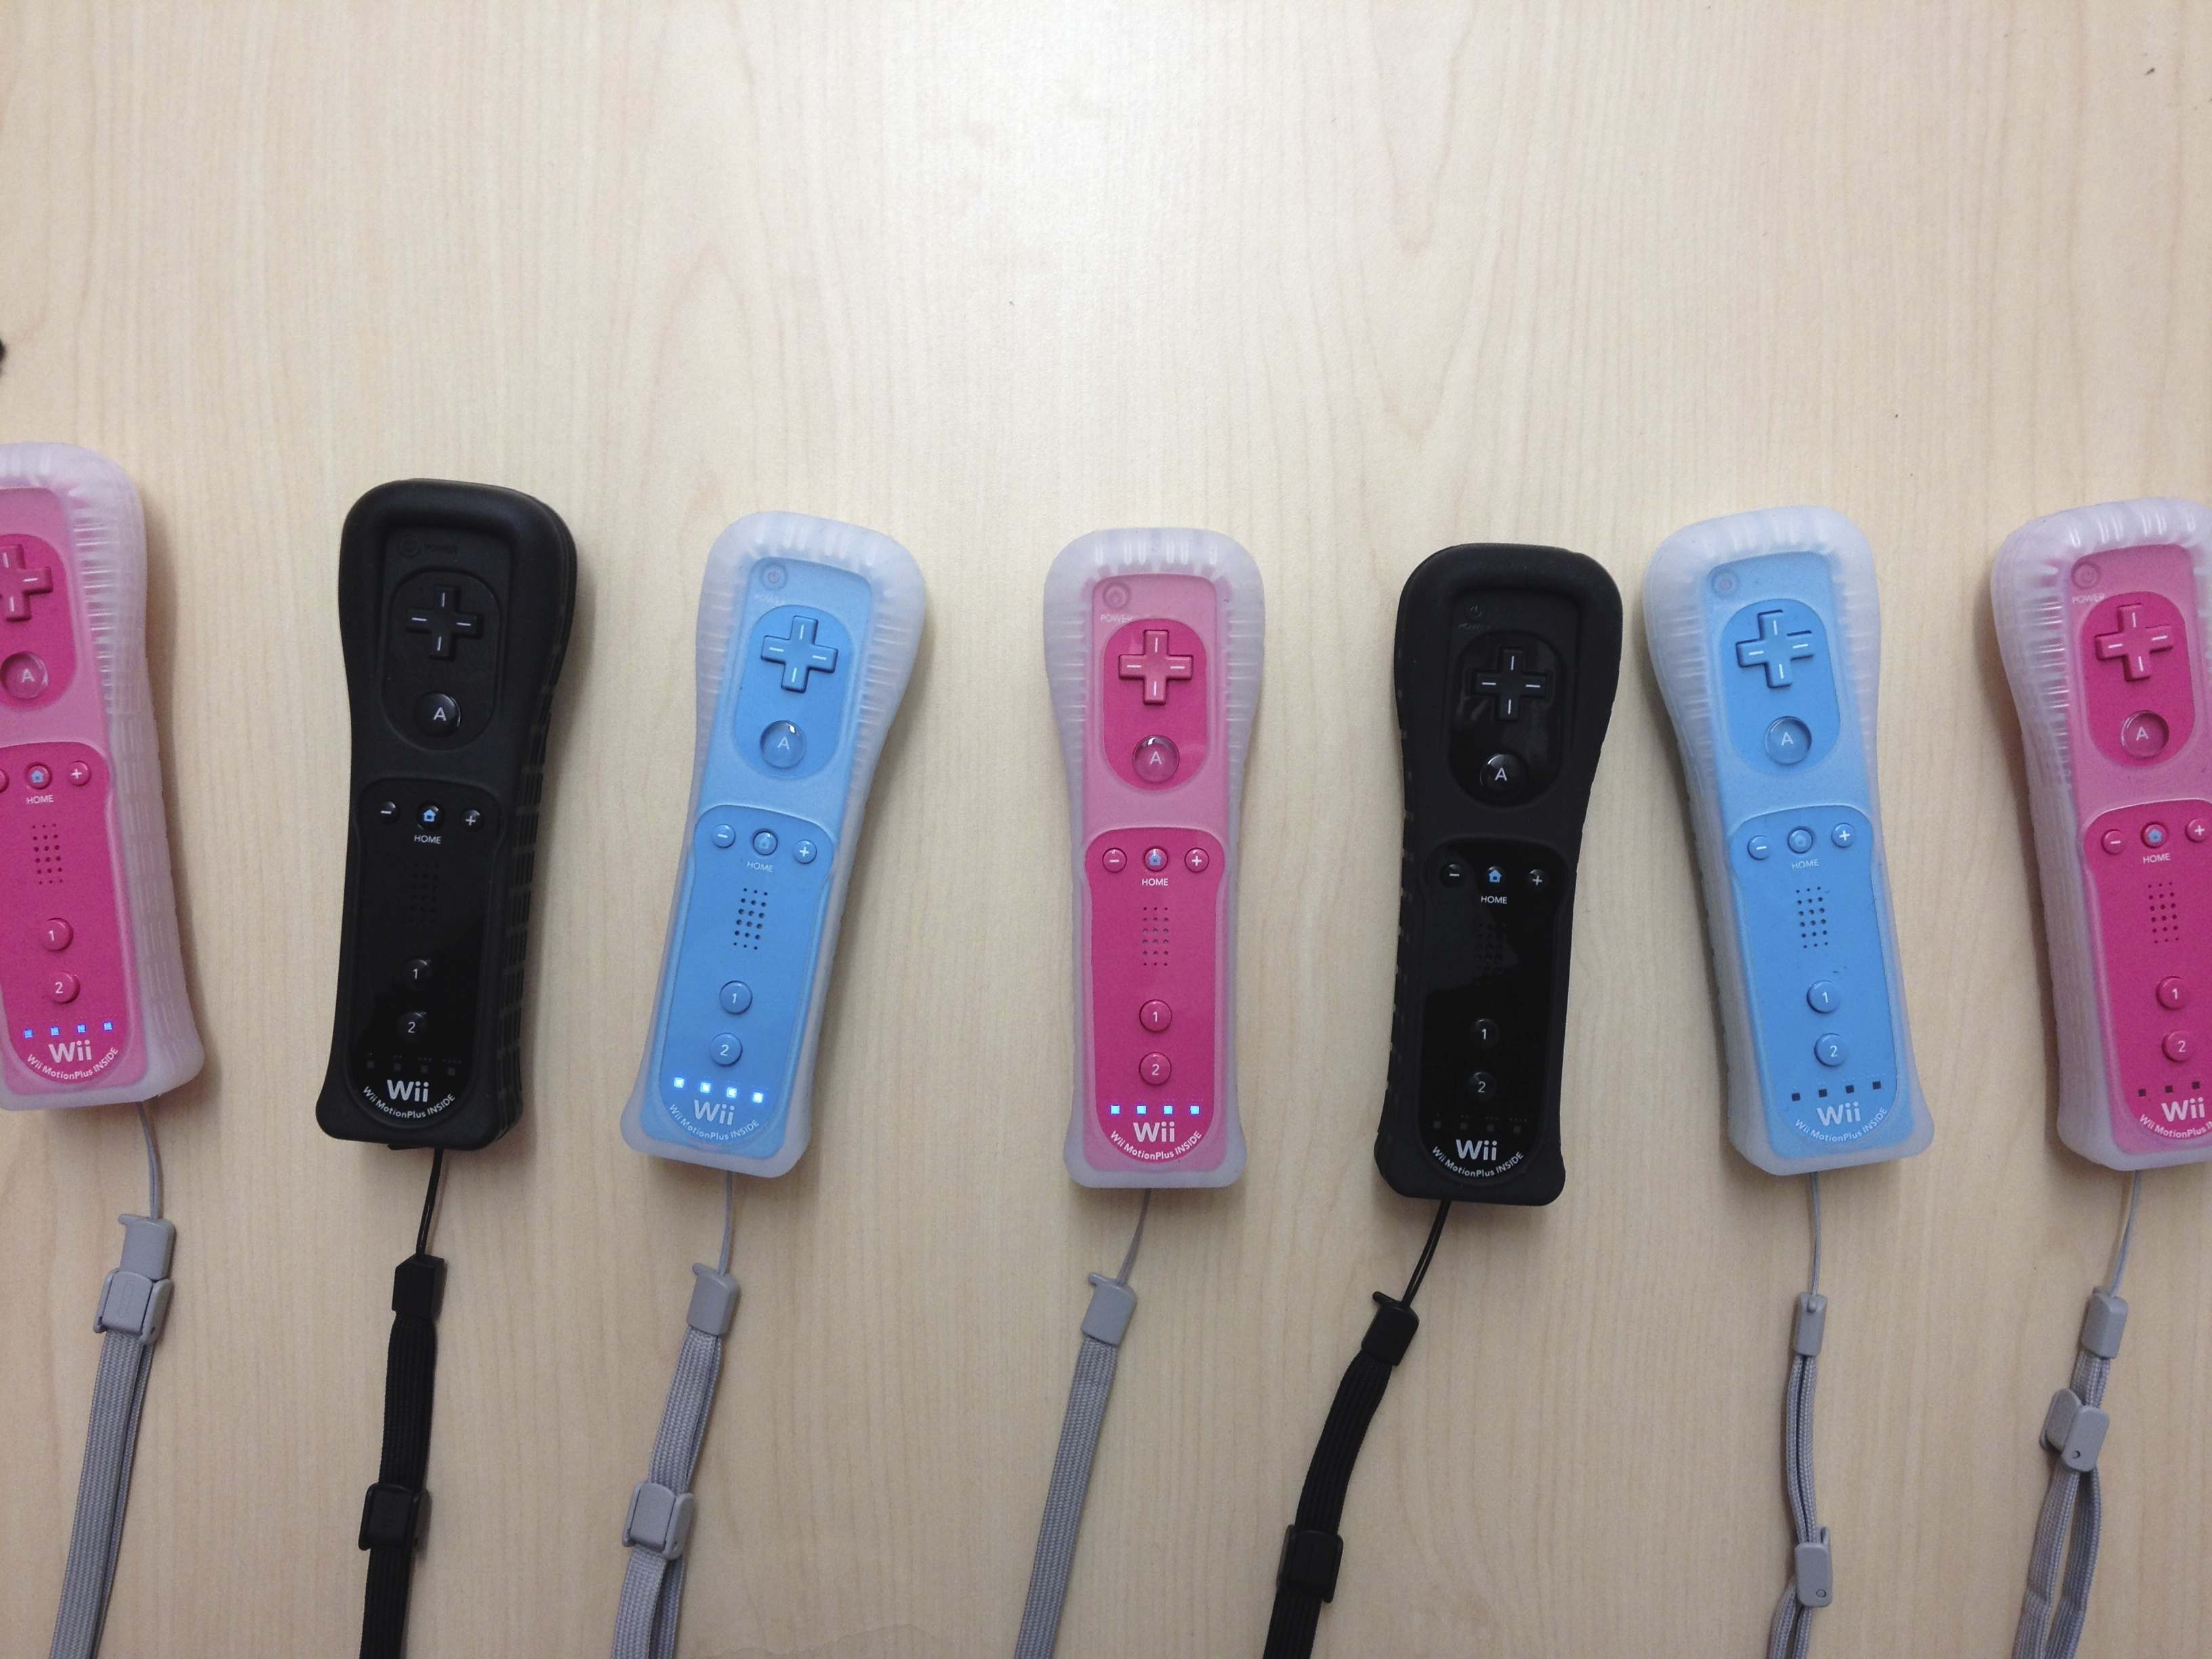
\includegraphics[height=0.32\textwidth]{wiimotes.jpg}}
	\hspace{0.1cm}
	\subfloat[Max patcher]{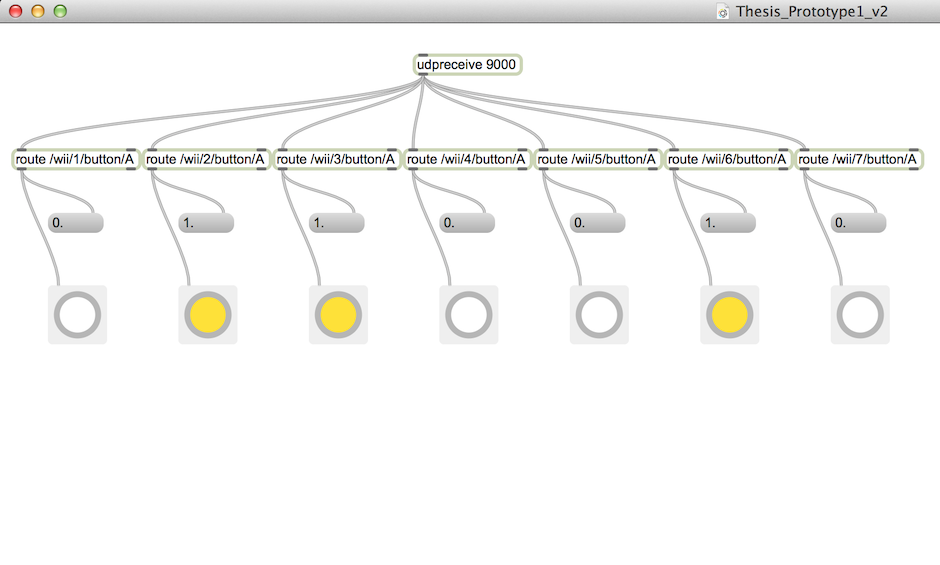
\includegraphics[height=0.32\textwidth]{multi_wii.png}}
	\caption{Testing simultaneous input from seven Wii controllers}

	\label{prototyping3}
\end{figure}

The next goal was to have multiple Wii controllers collaboratively manipulating a video in some way. I decided to create a patcher where users could ``vote" for how to control the video. In this case, I fed two video loops -- one monochrome clip of one person dancing and one colourful clip of multiple people dancing -- into a crossfader object. By pressing and holding the Left or Right buttons on their controllers, users can vote on which clip dominates the screen. In an effort to experiment with multiple motion data, I also incorporated a mechanism that lets users make their votes count double by shaking their controllers. Lastly, I packaged all of these programming objects into a ``sub-patcher," making the program more modular and readable. Figure \ref{prototyping4} shows the patcher running with three users.

\begin{figure}[t]
	\centering

	\subfloat[Main patcher]{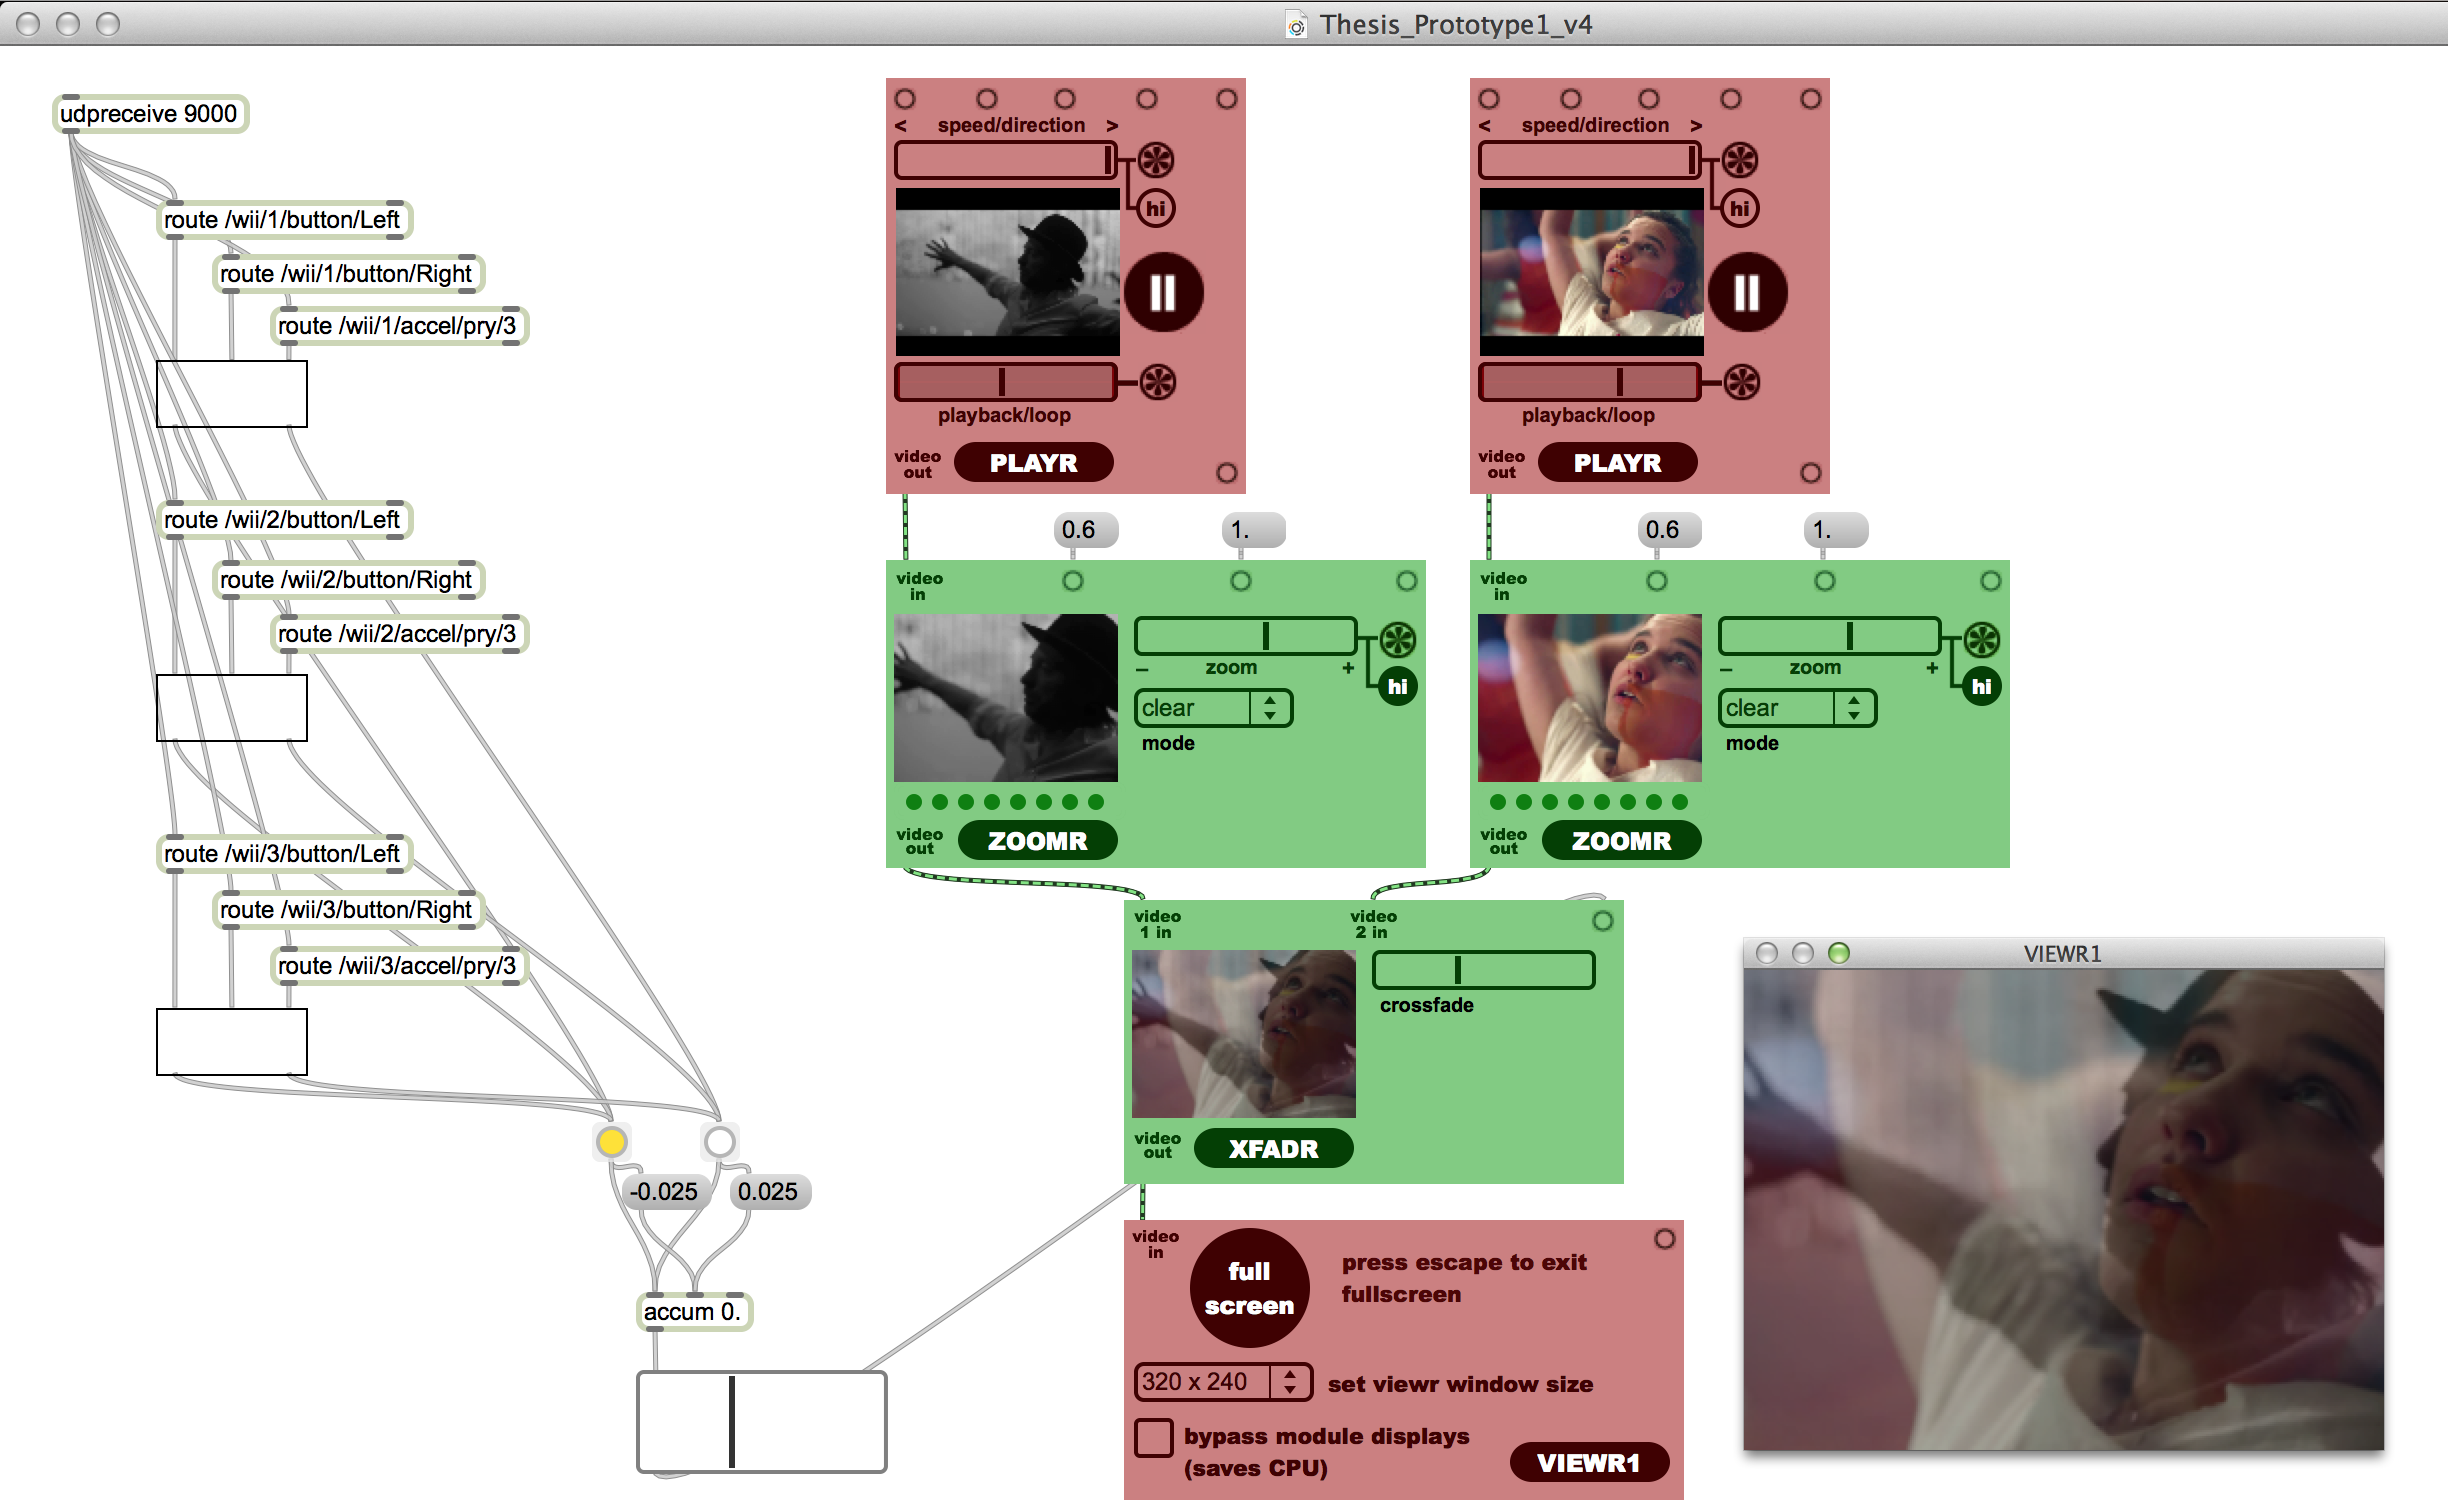
\includegraphics[height=0.3\textwidth]{threewii_voting.png}}
	\hspace{1cm}
	\subfloat[Sub-patcher]{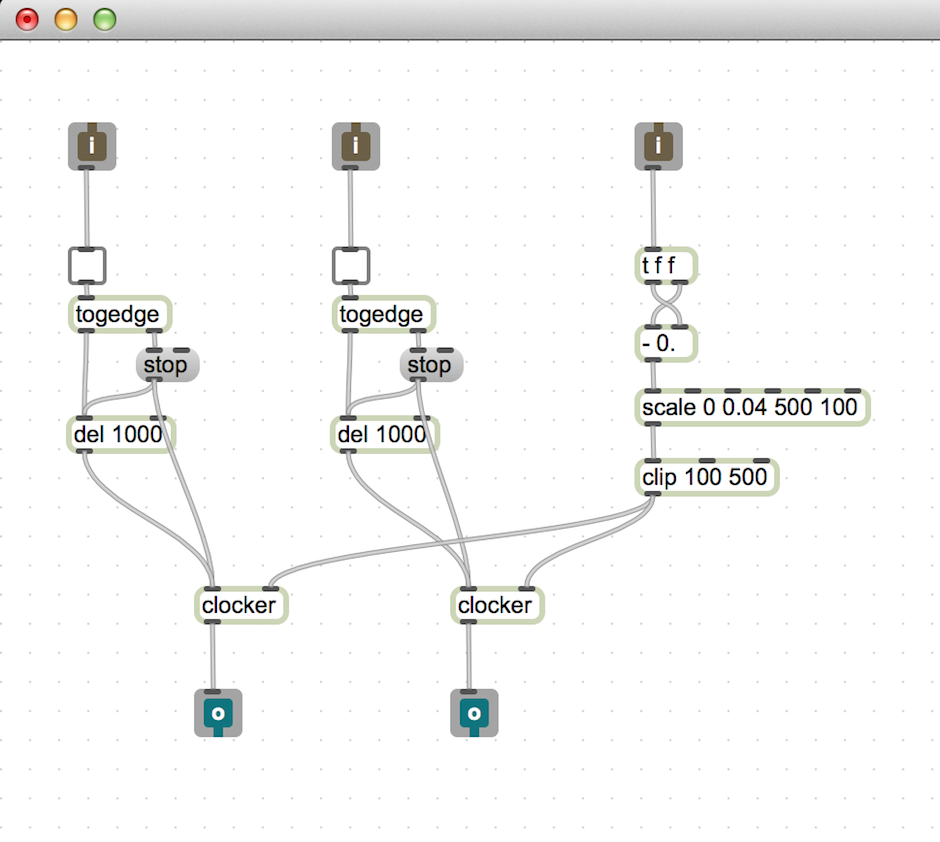
\includegraphics[height=0.3\textwidth]{threewii_voting_sub.png}}
	\caption{Video effect voting system with three users}

	\label{prototyping4}
\end{figure}

My next task was to create the VJ program for the performer in my scenario. I spent a lot of time experimenting with video effects in Max. I selected four effects objects that would allow the performer to rotate the image, control pixelation, enable a motion blur effect, and crossfade between two video loops. These are controlled by rotating the Wii controller, increasing the incline of the controller, pressing and holding the A button, and pressing the Left and Right buttons, respectively. An important part of programming this patcher was mapping the data from the controller to the effects controls. Values had to be carefully scaled and clipped in order for the user's movements to translate naturally to the effect they control. The patcher is pictured in Figure \ref{prototyping5}.

\begin{figure}[t]
	\centering

	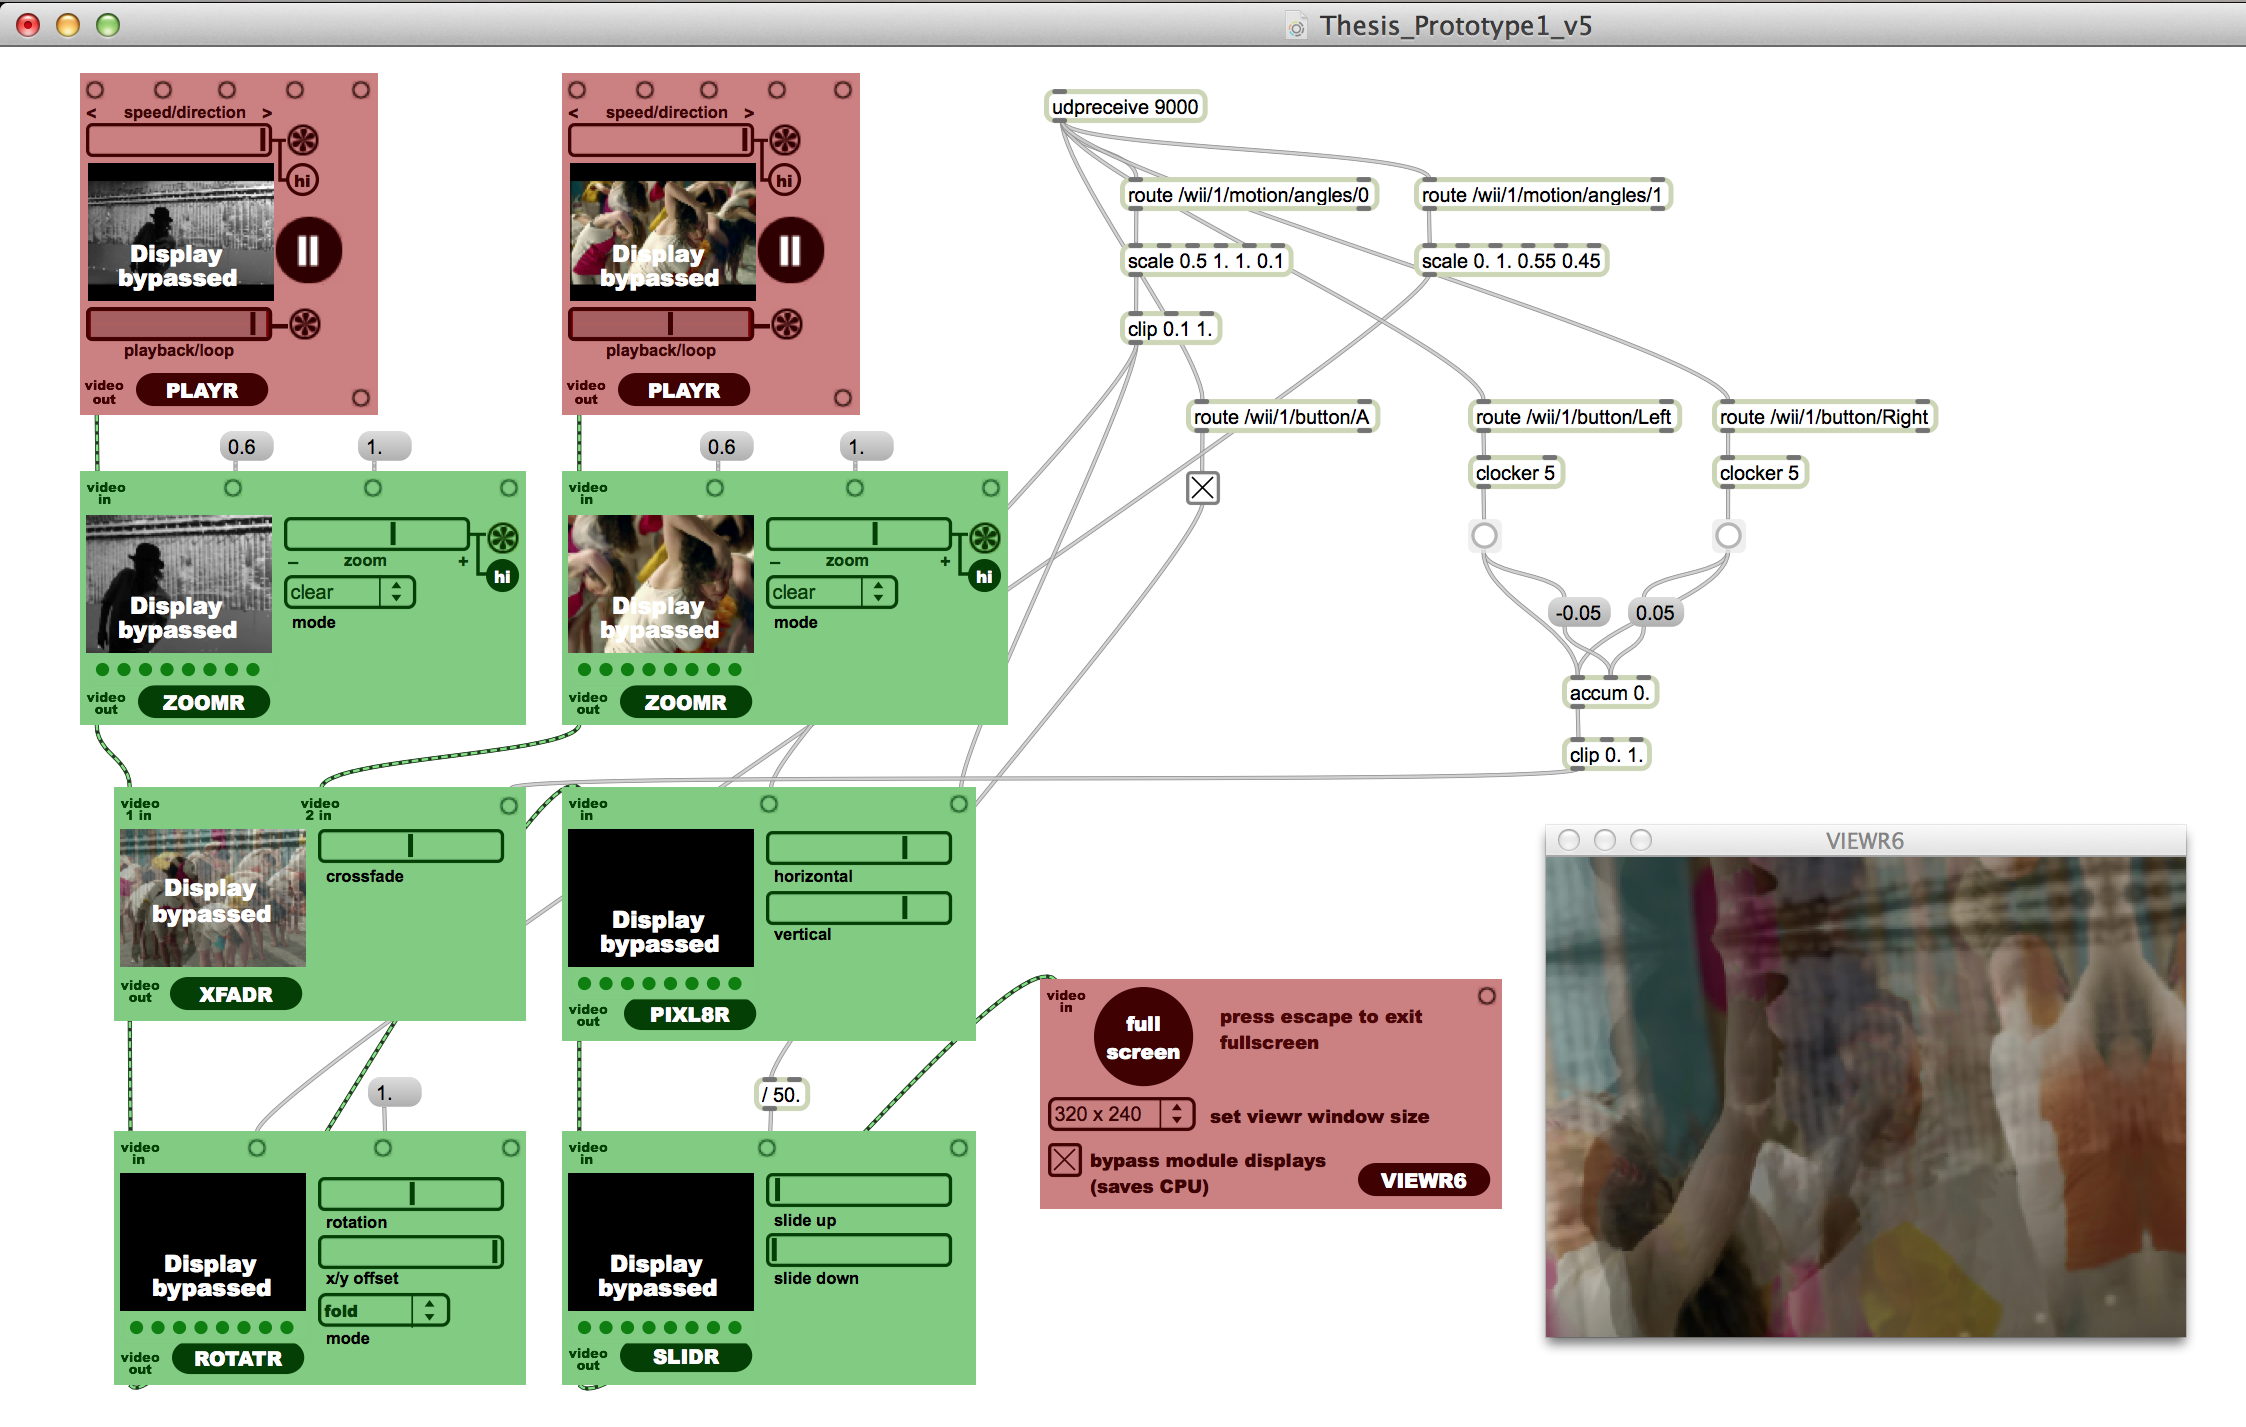
\includegraphics[height=0.3\textwidth]{wii_vj.png}
	\caption{Wii controller VJ system}

	\label{prototyping5}
\end{figure}

The results of the last two victories were finally combined to create my audience-performer interaction system (see Figure \ref{prototyping6}). Here, one user has the VJ controls described in the previous section. The audience voting system, however, is also implemented, allowing the other users to collaboratively control the crossfading of the two clips. Thus, as the performer simultaneously manipulates the two loops, the audience can decide which of them dominates the screen. Additionally, using the controller's B button, the performer has the ability to ``mute" the audience if their input is no longer desired. This stage required development of more sub-patchers to condense and modularize the program.

\begin{figure}[t]
	\centering

	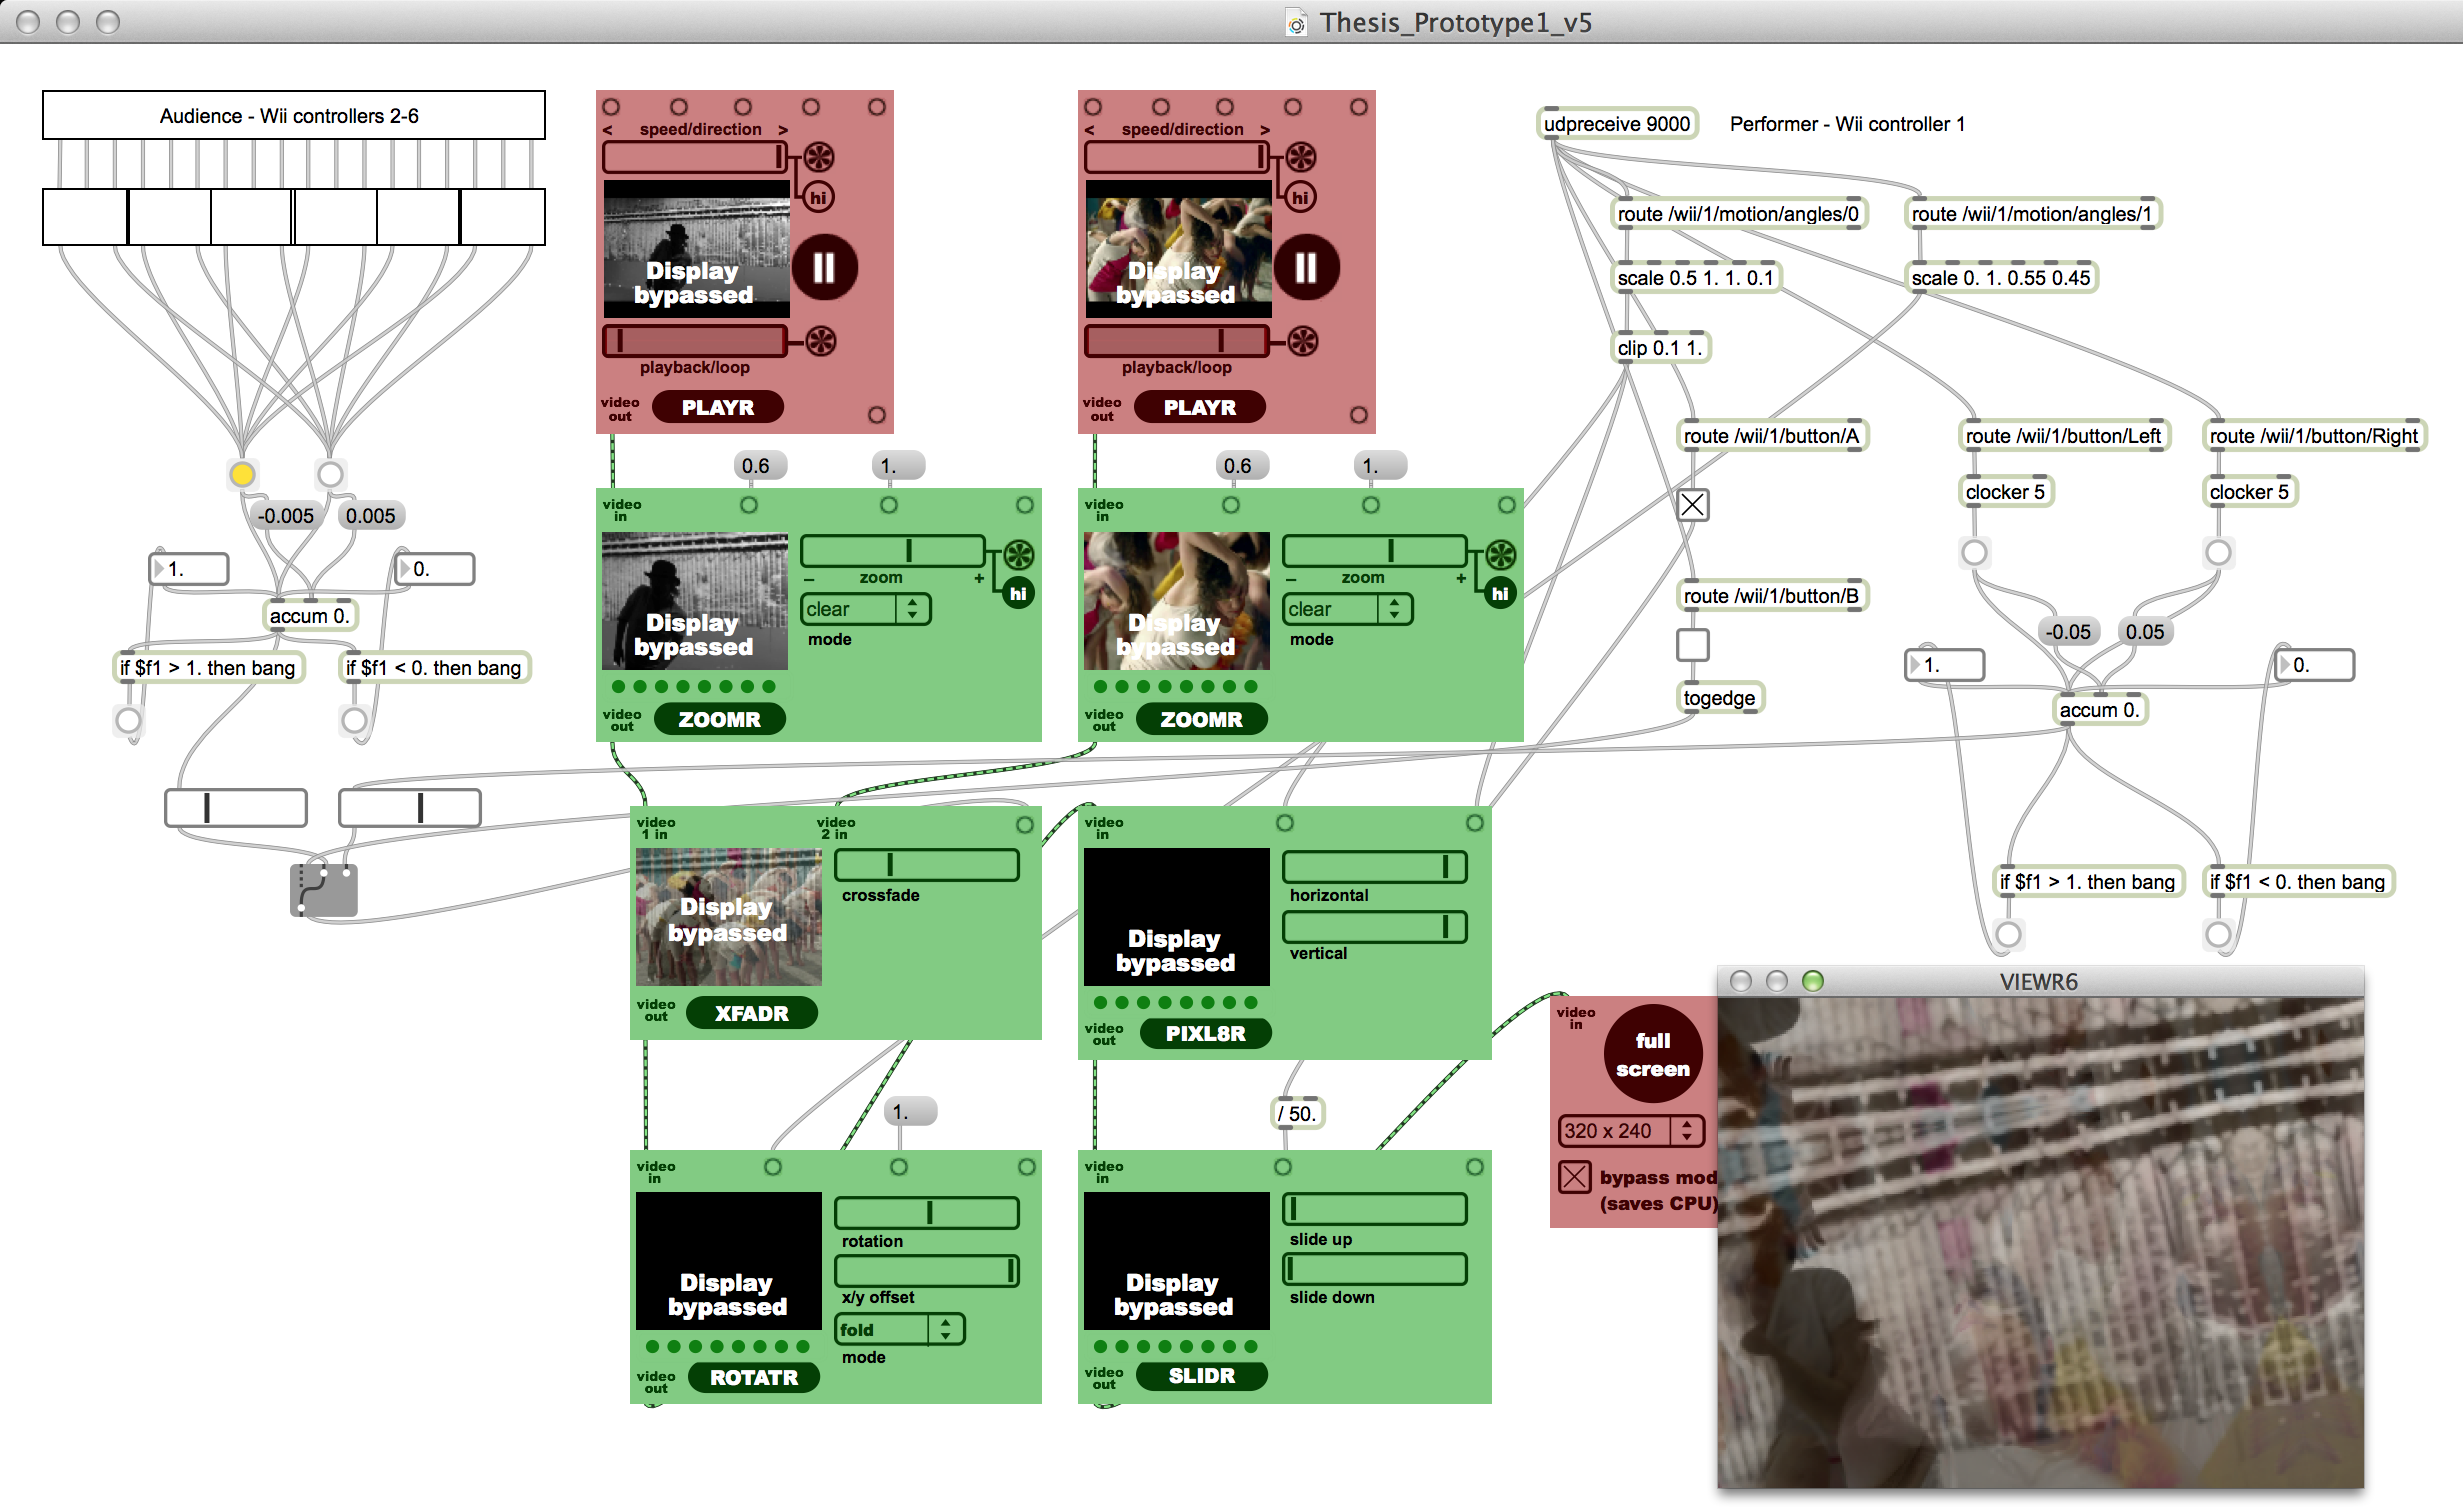
\includegraphics[height=0.3\textwidth]{vj_and_audience.png}
	\caption{Audience-performer interaction system}

	\label{prototyping6}
\end{figure}

\begin{itemize}
	\item I updated the look of the patcher, adding a dark background with light text.
	\item I added an auto-play function. This automatically flips through every round, playing each for a set amount of time.
	\item Added Lighters and Dance modes.
	\item Integrated video crossfade voting system within each mode.
	\item Added sub-patcher to lighten the processing load
	\item Polished off presentation mode.
\end{itemize}


\subsection{User Testing}

The first user testing was run at eLeo -- an interactive exhibit hosted by OCAD University. My prototype was set up in a room with a wall-sized projection. Here, my goal was to observe how users approached the technology and how they performed the various inputs.
% * My survey indicated that people attending smaller venues are more inclined to welcome new technologies at shows, so testing at a smaller venue isn't problematic


\section{Second Phase}

\subsection{Prototyping}

\subsection{User Testing}